\documentclass{article}

% Si el proyecto tiene neurips_2024.sty (plantilla oficial) se usa; si no,
% compila igual con margenes equivalentes.
\IfFileExists{neurips_2024.sty}{
  \usepackage[preprint]{neurips_2024}
}{
  \usepackage[letterpaper,margin=1in]{geometry}
  \usepackage[numbers,sort&compress]{natbib}
}

\usepackage[utf8]{inputenc}
\usepackage[T1]{fontenc}
\usepackage[spanish,es-noshorthands,es-nodecimaldot,es-tabla]{babel}
\usepackage{lmodern}
\usepackage{amsmath,amssymb}
\usepackage{booktabs}
\usepackage{graphicx}
\usepackage{xcolor}
\usepackage[hidelinks]{hyperref}
\usepackage{url}

\title{Detección de fauna en cámaras trampa con YOLO:\\
generalización a ubicaciones nuevas y monitoreo ecológico en CCT-20}

\author{%
  Nombre Apellido\\
  Maestría en Inteligencia Artificial, FIIS -- Universidad Nacional de Ingeniería\\
  Redes Neuronales y Aprendizaje Profundo, 2026-II\\
  \texttt{correo@uni.pe}
}

\begin{document}

\maketitle

\begin{abstract}
Las cámaras trampa generan millones de fotos, en su mayoría vacías, y revisarlas
a mano es el cuello de botella del monitoreo de fauna. Ajustamos YOLOv8 sobre
Caltech Camera Traps (CCT-20) y evaluamos por separado en cámaras vistas en
entrenamiento (\emph{cis}) y en cámaras nuevas (\emph{trans}). Agregar imágenes
vacías de otras ubicaciones como fondo reduce los falsos disparos a la mitad y
mejora el mAP. El modelo final alcanza mAP@0.5 de 0,721 en \emph{cis} y 0,459
en \emph{trans}; la caída es sobre todo de recall y se concentra en especies que
en entrenamiento aparecen en pocas cámaras. Una prueba de borrado del animal
descarta que el detector prediga especies a partir del fondo, mientras que
EigenCAM sobre el \emph{backbone} muestra que la representación sí está
dominada por la escena. Por último, un módulo de monitoreo basado en eventos,
aplicado a una cámara nunca vista, reproduce los patrones de actividad
nocturna de las especies comunes, pero pierde el 19\,\% de los eventos con
animal y casi no registra especies pequeñas.
\end{abstract}

% =====================================================================
\section{Introducción}
\label{sec:intro}

Una cámara trampa se dispara por movimiento o calor y deja una ráfaga de fotos.
En proyectos de monitoreo es habitual acumular cientos de miles de imágenes por
temporada, buena parte de ellas disparadas por viento, sombras o cambios de
luz y sin ningún animal. Los detectores de objetos prometen filtrar
las vacías y clasificar las especies, pero su desempeño suele reportarse en las
mismas cámaras con las que se entrenaron. Beery et al.~\cite{beery2018terra}
mostraron que en ubicaciones nuevas el rendimiento cae de forma marcada, porque
el fondo, el ángulo y la iluminación de cada cámara son casi constantes y el
modelo puede apoyarse en ellos.

En este trabajo estudiamos ese problema con un caso práctico: ajustar YOLO a
CCT-20 y preguntarnos qué tan útil sería en una cámara recién instalada. Las
contribuciones son: (i) un experimento controlado sobre el uso de imágenes
vacías como fondo; (ii) un análisis del AP por especie frente al desbalance de
clases; (iii) dos pruebas complementarias (borrado del animal y EigenCAM) para
distinguir entre ``aprendió el fondo'' y ``no reconoce al animal en un fondo
nuevo''; (iv) una medida de robustez por tamaño de caja y por oclusión
etiquetada manualmente; y (v) un módulo de monitoreo basado en reglas,
evaluado contra la revisión manual en una cámara no vista.

% =====================================================================
\section{Trabajo relacionado}
\label{sec:relacionado}

Norouzzadeh et al.~\cite{norouzzadeh2018} demostraron que las CNN pueden
identificar especies en Snapshot Serengeti con precisión cercana a la humana,
y Tabak et al.~\cite{tabak2019} llevaron la idea a modelos listos para usar en
ecología. MegaDetector~\cite{beery2019megadetector} cambió el enfoque: un
detector genérico de ``animal / persona / vehículo'' que filtra vacías y deja
la especie a otro modelo. No lo usamos porque no da la especie y porque entre
sus datos de entrenamiento figura Caltech Camera Traps, lo que contaminaría la
evaluación \emph{trans}. CCT-20 fue publicado precisamente para medir la
generalización a ubicaciones nuevas~\cite{beery2018terra}, y el fenómeno de
fondo que estudiamos es un caso del aprendizaje por atajos descrito por
Geirhos et al.~\cite{geirhos2020shortcut}. Para interpretabilidad partimos de
Grad-CAM~\cite{selvaraju2017gradcam} y usamos su variante sin gradientes,
EigenCAM~\cite{muhammad2020eigencam}, más fácil de aplicar a un detector.

% =====================================================================
\section{Datos}
\label{sec:datos}

Usamos CCT-20~\cite{beery2018terra}: 57\,864 fotos de 20 cámaras del suroeste
de Estados Unidos con 15 categorías (13 especies, \emph{car} y \emph{empty}),
en la versión reducida a 1024~px de lado mayor. Los splits oficiales separan
las cámaras: \texttt{train}, \texttt{cis\_val} y \texttt{cis\_test} comparten
las mismas 10 cámaras, mientras que \texttt{trans\_val} (1 cámara) y
\texttt{trans\_test} (9 cámaras) usan ubicaciones que no aparecen en
entrenamiento. Comprobamos que no hay cruce de ubicaciones entre
\texttt{train} y \texttt{trans\_test}.

La exploración mostró tres rasgos que condicionaron las decisiones.
\textbf{(1)} El split \texttt{train} no tiene ninguna imagen vacía, aunque en
test el 7--8\,\% de las fotos lo son. \textbf{(2)} El desbalance es extremo:
zarigüeya tiene 2\,514 cajas de entrenamiento y zorro, 5. Además, cada especie
suele concentrarse en pocas cámaras; por ejemplo, el 74\,\% de los gatos de
train proviene de una sola. \textbf{(3)} Entre el 55 y el 72\,\% de las fotos
son nocturnas (infrarrojas, en escala de grises), y alrededor del 10\,\% de las
cajas ocupan menos del 1\,\% de la imagen.

% =====================================================================
\section{Método}
\label{sec:metodo}

\subsection{Preparación del conjunto de detección}

\paragraph{Exclusiones.} Hay 1\,454 imágenes de train (y varios miles en test)
etiquetadas con una especie pero sin caja. No sirven como positivo, porque no
hay caja que aprender, ni como fondo, porque le enseñarían al modelo a ignorar
un animal presente; por eso se excluyen de todos los splits. También excluimos
la clase \emph{car}, que no es fauna, junto con sus imágenes. Las cajas se
recortan a los bordes de la imagen y se convierten a formato YOLO. El conjunto
final tiene 11\,431 imágenes de train, 4\,213 de validación (\texttt{cis\_val}
+ \texttt{trans\_val}), 13\,085 de \texttt{cis\_test} y 18\,698 de
\texttt{trans\_test}, con 14 especies.

\paragraph{Vacías como fondo.} Para compensar la ausencia de vacías en train,
descargamos 3\,000 fotos vacías de 106 ubicaciones de Caltech Camera Traps que
no forman parte de CCT-20, repartidas por ubicación para no sesgar hacia una
sola escena. En YOLO, una imagen con archivo de etiquetas vacío actúa como
ejemplo negativo. Usamos 2\,286 (20\,\% de las imágenes con animal), una
proporción que deja dominar a los positivos sin dejar de penalizar los falsos
disparos. Al venir de otras ubicaciones, no filtran información de las
cámaras de validación ni de test.

\subsection{Entrenamiento}

Partimos de pesos preentrenados en COCO~\cite{lin2014coco} y usamos la
implementación de Ultralytics~\cite{jocher2023yolov8} (v8.4.192, PyTorch 2.11,
una GPU Tesla T4 en Google Colab). Las decisiones principales fueron:

\begin{itemize}
  \item \textbf{Resolución 640~px.} Es el tamaño nativo de los pesos COCO y
  cabe en la T4 con lotes de 16--32. Se consideró 960~px por las cajas
  pequeñas, pero el costo de cómputo se duplicaba y se dejó como trabajo
  futuro.
  \item \textbf{Aumentos.} Mosaico (desactivado en las últimas 5 épocas para
  que el modelo vea imágenes completas), volteo horizontal ($p=0{,}5$), sin
  volteo vertical porque los animales no aparecen de cabeza, y saturación
  reducida ($h_s=0{,}4$ frente a 0,7 por defecto), ya que más de la mitad de
  las fotos son infrarrojas y una saturación agresiva genera colores que
  nunca ocurren.
  \item \textbf{Parada temprana} con paciencia de 10 épocas sobre el mAP de
  validación y semilla fija (42).
\end{itemize}

Realizamos tres experimentos: E1 (YOLOv8n, sin vacías, 30 épocas) y E2
(idéntico, con vacías) para aislar el efecto del fondo; y E3 (YOLOv8s, 50
épocas, con la mejor opción de E1/E2) como modelo final. El umbral de
confianza para los análisis por caja se eligió en validación con la curva
F1--confianza (Apéndice~\ref{app:f1}), nunca en test.

\subsection{Evaluación}

Reportamos mAP@0.5 y mAP@0.5:0.95 globales y por especie en
\texttt{cis\_test} y \texttt{trans\_test}. Como métrica propia, definimos la
\emph{tasa de falsos disparos}: el porcentaje de imágenes vacías con al menos
una detección de confianza $\geq 0{,}5$, que es lo que en la práctica decide
cuántas fotos vacías llegarían al revisor humano.

\paragraph{Prueba de borrado.} Sobre 300 imágenes con un solo animal por split,
cubrimos la caja (con un margen del 15\,\%) con el color medio de la imagen y
volvemos a detectar. Si la misma especie reaparece en la zona borrada o en otra
parte de la escena, la decisión se apoya en el contexto y no en el animal.

\paragraph{EigenCAM.} Grad-CAM~\cite{selvaraju2017gradcam} necesita un único
puntaje del que derivar gradientes, algo que un detector con cientos de cajas
candidatas no tiene de forma natural. EigenCAM~\cite{muhammad2020eigencam}
evita ese problema: proyecta las activaciones de una capa sobre su primera
componente principal. Lo implementamos sobre la salida del bloque SPPF (capa 9,
final del \emph{backbone}) y, además de las figuras, calculamos el \emph{lift}:
la fracción de la energía del mapa que cae dentro de las cajas reales dividida
entre la fracción de área que ocupan. Un lift de 1 significa que el mapa no
prefiere al animal sobre el resto de la imagen.

\paragraph{Tamaño y oclusión.} Para cada caja real calculamos si fue encontrada
con IoU $\geq 0{,}5$ y la especie correcta (recall) o con cualquier especie
(\emph{localizada}). Usamos recall y no AP por grupo porque un falso positivo
no tiene tamaño ni oclusión real a la que asignarse. El tamaño se agrupa por
área relativa ($<1$\,\%, 1--5\,\%, $>5$\,\%). Para la oclusión, que CCT-20 no
anota, etiquetamos a mano 150 cajas por split de test sobre las imágenes a
resolución completa, en tres niveles (bajo $<25$\,\%, medio 25--60\,\%, alto
$>60$\,\% del animal oculto). Re-etiquetamos a ciegas 50 de ellas y medimos la
autoconsistencia con $\kappa$ de Cohen~\cite{cohen1960kappa}.

\subsection{Módulo de monitoreo ecológico}

Un ecólogo no necesita cajas por foto, sino eventos, especies e individuos por
cámara y por periodo. El módulo agrega las detecciones de una cámara con cinco
reglas:
\textbf{R1}~una detección cuenta si su confianza es $\geq 0{,}5$;
\textbf{R2}~las fotos separadas por $\leq 60$~s forman un evento (se usa la
hora de la foto y no el identificador de secuencia, porque en campo solo se
tiene la hora);
\textbf{R3}~la especie del evento es la de mayor suma de confianzas;
\textbf{R4}~los individuos de una especie son el máximo de detecciones en un
mismo fotograma, no la suma, porque el mismo animal aparece en varias fotos de
la ráfaga;
\textbf{R5}~un evento sin detecciones es una activación vacía.
Aplicando las mismas reglas a las etiquetas reales obtenemos el reporte que
daría una revisión manual, lo que permite medir el error en las unidades que
importan al usuario.

% =====================================================================
% Seccion de resultados (Pregunta 3). Pensada para la plantilla NeurIPS con
% \usepackage[utf8]{inputenc}, \usepackage[spanish]{babel}, booktabs y graphicx.
% Las figuras se copian desde MyDrive/pregunta3_runs/E3_principal/ a informe/figuras/.

\section{Resultados}
\label{sec:resultados}

Todas las cifras de test se obtuvieron una sola vez con el modelo final (E3) y
umbrales fijados de antemano en validación. La curva F1--confianza de
validación alcanza su máximo ($F1=0{,}73$) en $0{,}45$ y es prácticamente plana
entre $0{,}4$ y $0{,}6$; por eso se usó $\text{conf}=0{,}5$ en los análisis por
caja, por tamaño y de monitoreo.

\subsection{Ajuste fino y efecto de las imágenes vacías}

El split \texttt{train} de CCT-20 no contiene imágenes vacías, aunque en campo
la mayoría de los disparos lo son. Para medir si conviene enseñarle el fondo al
modelo, entrenamos dos YOLOv8n idénticos (640~px, 30 épocas, misma semilla) que
solo difieren en que E2 agrega 2\,286 imágenes vacías (20\,\% de las imágenes
con animal) tomadas de ubicaciones que no pertenecen a CCT-20, de modo que no
filtran información de las cámaras de validación ni de test.

\begin{table}[h]
  \centering
  \caption{Efecto de las imágenes vacías en validación (\texttt{cis\_val} +
  \texttt{trans\_val}, 4\,213 imágenes). ``Falsos disparos'': porcentaje de
  imágenes vacías con al menos una detección de confianza $\geq 0{,}5$.}
  \label{tab:vacias}
  \begin{tabular}{lcccc}
    \toprule
    Experimento & mAP@0.5 & mAP@0.5:0.95 & Falsos disp. cis & Falsos disp. trans \\
    \midrule
    E1: YOLOv8n, sin vacías   & 0,730 & 0,486 & 6,0\,\% & 8,2\,\% \\
    E2: YOLOv8n, +20\,\% vacías & 0,748 & 0,514 & 3,4\,\% & 4,9\,\% \\
    E3: YOLOv8s, +20\,\% vacías & 0,784 & 0,539 & -- & -- \\
    \bottomrule
  \end{tabular}
\end{table}

Agregar vacías no solo reduce casi a la mitad los falsos disparos, que era lo
esperado, sino que también sube el mAP (+1,8 puntos en mAP@0.5 y +2,8 en
mAP@0.5:0.95). Nuestra lectura es que, sin ejemplos negativos de escena
completa, el modelo aprende a marcar como animal ciertas texturas del fondo
(troncos, rocas, sombras) y esos falsos positivos penalizan la precisión. Con
base en esto, el modelo principal E3 se entrenó sobre el conjunto con vacías,
cambiando a YOLOv8s y 50 épocas. El entrenamiento se detuvo por
\emph{early stopping} en la época 44 (mejor época: 34).

\subsection{Desempeño por especie y efecto del desbalance}

\begin{table}[h]
  \centering
  \caption{AP por especie en test, ordenado por número de cajas en
  entrenamiento. $n$: instancias en cada test. Ciervo no aparece en
  \texttt{trans\_test}.}
  \label{tab:especies}
  \small
  \begin{tabular}{lrrrrrrr}
    \toprule
     & & \multicolumn{3}{c}{\texttt{cis\_test}} & \multicolumn{3}{c}{\texttt{trans\_test}} \\
    \cmidrule(lr){3-5}\cmidrule(lr){6-8}
    Especie & Cajas train & $n$ & AP50 & AP50:95 & $n$ & AP50 & AP50:95 \\
    \midrule
    zorro (fox)          &     5 &     2 & 0,224 & 0,184 &     1 & 0,000 & 0,000 \\
    tejón (badger)       &     9 &     4 & 0,003 & 0,002 &    15 & 0,141 & 0,098 \\
    ciervo (deer)        &    44 &   140 & 0,504 & 0,327 &     0 & --    & --    \\
    zorrillo (skunk)     &   214 &   162 & 0,947 & 0,629 &   273 & 0,818 & 0,519 \\
    roedor (rodent)      &   264 &   146 & 0,811 & 0,451 &    26 & 0,003 & 0,001 \\
    ave (bird)           &   560 &   752 & 0,622 & 0,327 &   180 & 0,094 & 0,049 \\
    lince (bobcat)       &   684 &   772 & 0,863 & 0,608 & 1\,979 & 0,703 & 0,470 \\
    perro (dog)          &   769 &   725 & 0,765 & 0,527 &   961 & 0,707 & 0,476 \\
    mapache (raccoon)    & 1\,030 &   981 & 0,932 & 0,616 & 4\,803 & 0,780 & 0,509 \\
    ardilla (squirrel)   & 1\,037 &   510 & 0,724 & 0,393 &   782 & 0,296 & 0,162 \\
    gato (cat)           & 1\,170 & 1\,528 & 0,933 & 0,626 & 1\,366 & 0,293 & 0,192 \\
    coyote               & 1\,371 & 1\,182 & 0,922 & 0,699 & 1\,902 & 0,608 & 0,427 \\
    conejo (rabbit)      & 2\,278 & 1\,559 & 0,901 & 0,570 &   722 & 0,642 & 0,342 \\
    zarigüeya (opossum)  & 2\,514 & 4\,010 & 0,948 & 0,525 & 4\,663 & 0,885 & 0,470 \\
    \midrule
    \textbf{mAP}         &       & 12\,473 & \textbf{0,721} & \textbf{0,463} & 17\,673 & \textbf{0,459} & \textbf{0,286} \\
    \bottomrule
  \end{tabular}
\end{table}

La Tabla~\ref{tab:especies} muestra que el desbalance se nota sobre todo en los
extremos. Las dos especies con menos de diez cajas de entrenamiento (zorro y
tejón) no pasan de 0,22 de AP50, mientras que las cuatro especies con más de
1\,100 cajas superan 0,90 de AP50 en \texttt{cis\_test}. La correlación de
Spearman entre AP50 y número de cajas es $\rho=0{,}68$ ($p=0{,}008$, 14
especies) en \texttt{cis\_test} y baja a $\rho=0{,}49$ ($p=0{,}09$, 13 especies)
en \texttt{trans\_test} (Figura~\ref{fig:desbalance}). Hay que leer con cautela
las especies raras: con 2 o 4 instancias de test, un solo acierto o fallo mueve
el AP de 0 a 0,5, de modo que lo único que podemos afirmar es que el modelo no
aprendió a detectarlas de forma confiable.

El desbalance, sin embargo, no explica las peores caídas en cámaras nuevas. Gato
(1\,170 cajas) cae de 0,93 a 0,29 y ardilla (1\,037) de 0,72 a 0,30, mientras que
zorrillo, con solo 214 cajas, se mantiene en 0,82. Esa es la razón de que la
correlación se debilite en \texttt{trans\_test}: fuera de las cámaras de
entrenamiento, la cantidad de datos importa menos que la diversidad de escenas
en las que aparece cada especie.

\begin{figure}[h]
  \centering
  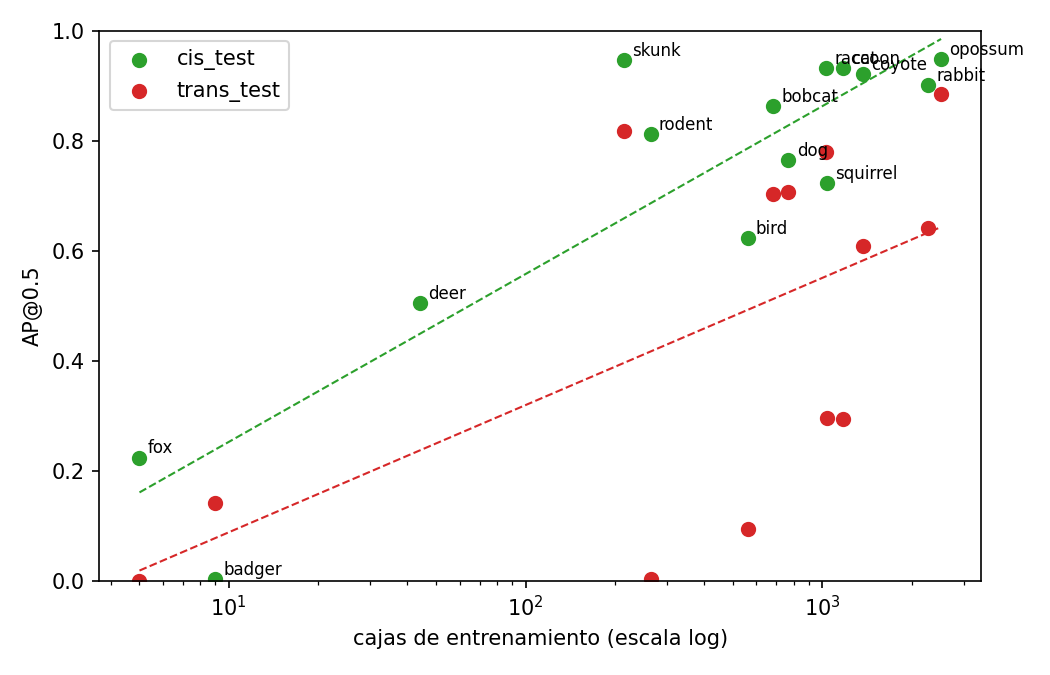
\includegraphics[width=0.7\linewidth]{figuras/ap_vs_cajas_train.png}
  \caption{AP50 por especie frente al número de cajas de entrenamiento (escala
  logarítmica). Verde: \texttt{cis\_test}; rojo: \texttt{trans\_test}. Las
  líneas discontinuas son solo una guía visual.}
  \label{fig:desbalance}
\end{figure}

\subsection{Generalización a ubicaciones nuevas y aprendizaje del fondo}

Entre \texttt{cis\_test} y \texttt{trans\_test} el mAP@0.5 cae de 0,721 a 0,459
(-26 puntos) y el mAP@0.5:0.95 de 0,463 a 0,286. La caída viene sobre todo del
recall (0,66 $\rightarrow$ 0,42); la precisión baja menos (0,87 $\rightarrow$
0,67) y la tasa de falsos disparos en las vacías de test casi no cambia (3,6\,\%
en cis frente a 4,3\,\% en trans). En otras palabras, en una cámara nueva el
modelo deja de ver animales mucho más de lo que inventa.

Para saber si el modelo aprendió el fondo de las cámaras de entrenamiento como
atajo, aplicamos dos pruebas sobre 300 imágenes con un solo animal por split.

\paragraph{Prueba de borrado.} Tapamos la caja del animal (con un margen de
15\,\%) con el color medio de la imagen y volvimos a detectar. Si el modelo
dependiera del contexto, debería seguir prediciendo la especie aunque el animal
ya no esté. No ocurrió: en ningún caso la misma especie reapareció en la zona
borrada, y solo hubo 1 de 300 casos en \texttt{cis\_test} (un conejo) y 2 de 300
en \texttt{trans\_test} (dos ardillas) en que la especie se predijo en otra parte
de la escena. El resultado es el mismo si nos quedamos solo con las imágenes que
el modelo había detectado bien al principio (250 en cis y 210 en trans).

\paragraph{EigenCAM.} Implementamos EigenCAM sobre la salida del bloque SPPF
(capa 9, final del \emph{backbone}) y medimos qué fracción de la energía del
mapa cae dentro de las cajas reales, normalizada por el área que ocupan
(\emph{lift}; 1 equivale a no preferir al animal sobre el resto de la imagen).
El lift mediano fue de 0,05--0,08 en todos los grupos, incluidas las detecciones
correctas (Tabla~\ref{tab:eigencam}). Visualmente, el mapa se concentra en
estructuras grandes de la escena (la franja de vegetación del horizonte, el
borde del camino) y no en el animal (Figura~\ref{fig:eigencam}).

\begin{table}[h]
  \centering
  \caption{EigenCAM en la capa 9: fracción de energía dentro de las cajas
  reales, fracción de área que ocupan y lift mediano (150 imágenes por split).}
  \label{tab:eigencam}
  \begin{tabular}{llrccc}
    \toprule
    Split & Detección correcta & $n$ & Energía en cajas & Área de cajas & Lift mediano \\
    \midrule
    \texttt{cis\_test}   & sí  & 124 & 0,022 & 0,048 & 0,059 \\
                         & no  &  26 & 0,060 & 0,068 & 0,083 \\
    \texttt{trans\_test} & sí  &  97 & 0,022 & 0,033 & 0,047 \\
                         & no  &  53 & 0,111 & 0,137 & 0,085 \\
    \bottomrule
  \end{tabular}
\end{table}

\begin{figure}[h]
  \centering
  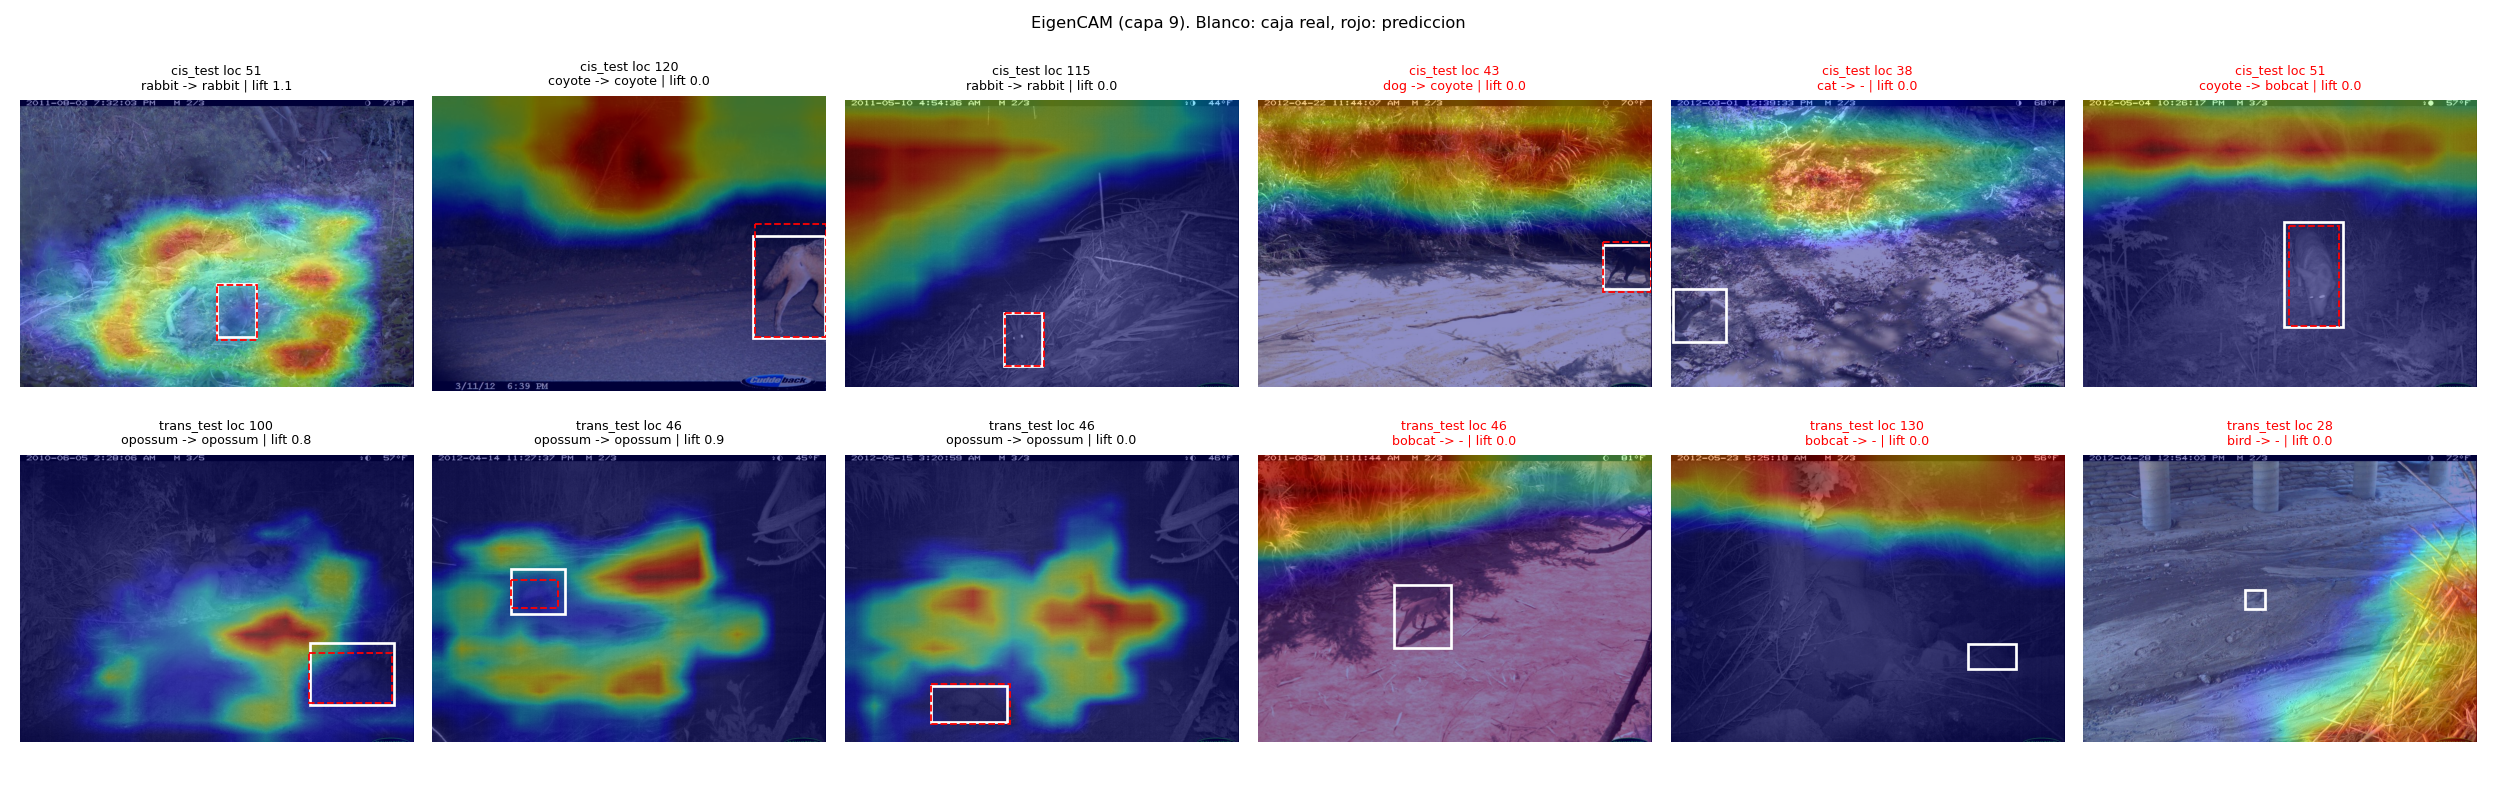
\includegraphics[width=\linewidth]{figuras/eigencam_ejemplos.png}
  \caption{EigenCAM (capa 9). Fila superior: \texttt{cis\_test}; inferior:
  \texttt{trans\_test}. Blanco: caja real; rojo discontinuo: predicción. Títulos
  en rojo: detecciones fallidas.}
  \label{fig:eigencam}
\end{figure}

Las dos pruebas parecen contradecirse, pero responden preguntas distintas.
EigenCAM proyecta las activaciones sobre su primera componente principal, es
decir, sobre la dirección de mayor varianza espacial; en una cámara fija, esa
varianza la domina la estructura de la escena, no un animal que en esta muestra
ocupa entre el 3 y el 14\,\% de la imagen. El mapa muestra entonces que la
representación del \emph{backbone} está dominada por el fondo, pero no que la
decisión de la cabeza de detección dependa de él, y la prueba de borrado indica
que no depende. Concluimos que la caída cis$\rightarrow$trans no se explica por
un atajo del tipo ``esta cámara $\Rightarrow$ esta especie'', sino por
animales que el modelo no reconoce cuando cambian el fondo, el ángulo y la
iluminación. Esto es coherente con que la pérdida sea de recall y no de
precisión.

La distribución de las especies entre las cámaras de entrenamiento apoya esta
lectura, aunque solo de forma parcial. Las tres especies que más caen en
\texttt{trans\_test} son las más concentradas en train: el 90\,\% de las cajas
de roedor, el 88\,\% de las de gato y el 81\,\% de las de ave provienen de solo
dos de las diez cámaras (el 74\,\% de los gatos, de la cámara 38). El modelo vio
a esas especies casi siempre sobre el mismo fondo y con el mismo ángulo. En el
otro extremo, zorrillo está repartido en siete cámaras (las dos principales
suman el 57\,\%) y conserva 0,82 de AP50. Sin embargo, la relación no es
general: considerando las 11 especies con datos suficientes, la correlación
entre concentración y caída es débil ($\rho=0{,}33$, $p=0{,}32$). Ardilla está
bien repartida y aun así cae 43 puntos, y zarigüeya está concentrada pero su
abundancia la protege.
% Si se repite EigenCAM en una capa del cuello (--capa 15), comparar aqui.

\subsection{Robustez al tamaño y a la oclusión}

Medimos el recall por caja (IoU $\geq 0{,}5$ y especie correcta) y, por
separado, si la caja fue \emph{localizada} con cualquier especie. Así se
distinguen los errores de localización de los de clasificación. Los cortes de
tamaño se fijaron según el área relativa de la caja: pequeña $<1$\,\%, mediana
1--5\,\% y grande $>5$\,\%.

\begin{table}[h]
  \centering
  \caption{Recall y fracción localizada por tamaño de caja ($\text{conf}\geq0{,}5$).}
  \label{tab:tamano}
  \begin{tabular}{lrccrcc}
    \toprule
     & \multicolumn{3}{c}{\texttt{cis\_test}} & \multicolumn{3}{c}{\texttt{trans\_test}} \\
    \cmidrule(lr){2-4}\cmidrule(lr){5-7}
    Tamaño & $n$ & Recall & Localizada & $n$ & Recall & Localizada \\
    \midrule
    Pequeña ($<1$\,\%)  & 1\,149 & 0,560 & 0,591 & 1\,924 & 0,346 & 0,376 \\
    Mediana (1--5\,\%)  & 8\,929 & 0,844 & 0,895 & 12\,183 & 0,713 & 0,788 \\
    Grande ($>5$\,\%)   & 2\,395 & 0,823 & 0,869 & 3\,566 & 0,462 & 0,637 \\
    \bottomrule
  \end{tabular}
\end{table}

Los animales pequeños son el punto débil esperado: a 640~px, una caja del 1\,\%
de una imagen de 1024 px queda en unos 60$\times$40 píxeles, y en esos casos casi
todos los fallos son de localización (recall y localizada casi iguales). Lo
inesperado está en las cajas grandes de \texttt{trans\_test}: el recall cae a
0,46, por debajo del de las medianas, mientras que el 64\,\% de esas cajas sí se
localiza. Es decir, el modelo encuentra al animal pero se equivoca de especie.
Nuestra hipótesis es que se trata de animales muy cerca del lente, cortados por
el borde del encuadre o sobreexpuestos por el flash infrarrojo, situaciones en
las que se pierden la silueta y la textura que distinguen, por ejemplo, a un
gato de un lince.
% TODO: confirmar mirando 10-20 cajas grandes de trans_test con recall=False y
% localizada=True (tamano_oclusion/cajas_emparejadas.csv).

% TODO: completar con etiquetas_oclusion.csv (300 cajas, 3 niveles) y el kappa
% de autoconsistencia sobre las 50 repetidas.
\paragraph{Oclusión.} \textit{[Pendiente: recall por nivel de oclusión (bajo
$<25$\,\%, medio 25--60\,\%, alto $>60$\,\%) sobre 150 cajas por split etiquetadas
manualmente, y $\kappa$ de autoconsistencia sobre 50 cajas re-etiquetadas a
ciegas.]}

\subsection{Módulo de monitoreo en una cámara no vista}

% TODO: \label{sec:metodo} debe existir en la seccion de metodo del informe.
Aplicamos el módulo de monitoreo (reglas R1--R5, sección~\ref{sec:metodo}) a la
cámara 46 de \texttt{trans\_test}, la de más fotos entre las cámaras que el
modelo nunca vio: 6\,276 fotos entre mayo de 2011 y junio de 2012, agrupadas en
1\,383 eventos. El mismo procedimiento aplicado a las etiquetas reales da el
reporte que se obtendría revisando las fotos a mano, y sirve de referencia
(Tabla~\ref{tab:monitoreo} y Figura~\ref{fig:actividad}).

\begin{figure}[t]
  \centering
  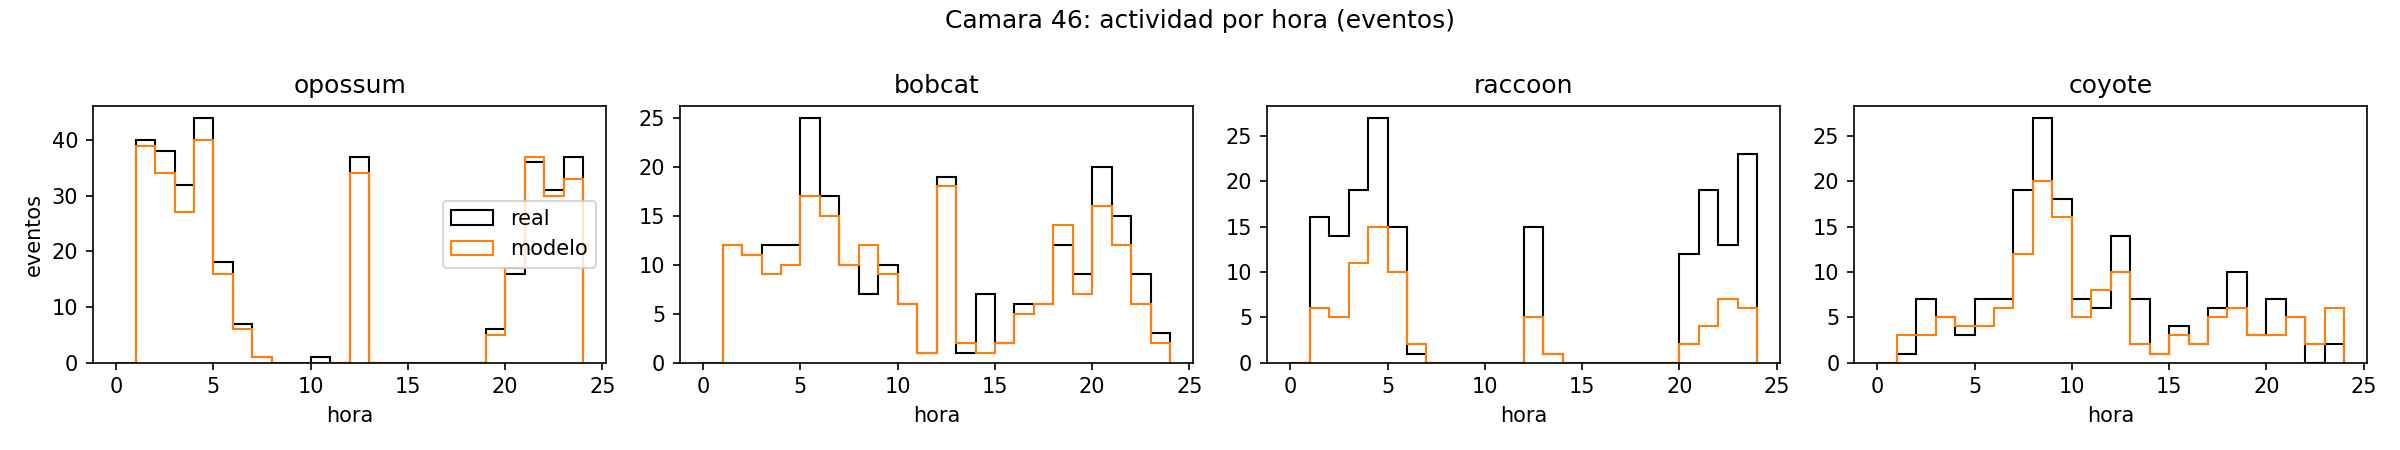
\includegraphics[width=\linewidth]{figuras/actividad_hora_camara46.png}
  \caption{Cámara 46 (no vista en entrenamiento): eventos por hora del día para
  las cuatro especies más frecuentes, según el modelo (naranja) y según la
  revisión manual (negro).}
  \label{fig:actividad}
\end{figure}

\begin{table}[h]
  \centering
  \caption{Reporte de la cámara 46: modelo frente a revisión manual.}
  \label{tab:monitoreo}
  \begin{tabular}{lcc}
    \toprule
    Indicador & Modelo & Real \\
    \midrule
    Fotos vacías                         & 55,5\,\% & 11,6\,\% \\
    Eventos vacíos                       & 31,8\,\% & 16,1\,\% \\
    Especies registradas                 & 10 & 12 \\
    Acierto de especie por evento        & \multicolumn{2}{c}{75,0\,\%} \\
    Eventos con animal marcados vacíos   & \multicolumn{2}{c}{221 de 1\,161 (19\,\%)} \\
    Eventos vacíos marcados con animal   & \multicolumn{2}{c}{3} \\
    \midrule
    \% nocturno zarigüeya / mapache      & 0,87 / 0,89 & 0,87 / 0,90 \\
    \% nocturno zorrillo / lince         & 0,76 / 0,50 & 0,81 / 0,55 \\
    Eventos zarigüeya / lince / coyote   & 319 / 203 / 134 & 344 / 232 / 168 \\
    Eventos gato / ave / roedor          & 55 / 3 / 0 & 5 / 25 / 14 \\
    \bottomrule
  \end{tabular}
\end{table}

Agrupar en eventos compensa buena parte de los errores por foto: aunque el
modelo deja sin detección a más de la mitad de las fotos, basta con que acierte
en una foto de la ráfaga para registrar el evento, y la diferencia en eventos
vacíos se reduce a la mitad (31,8\,\% frente a 16,1\,\%). Para las especies
abundantes, los indicadores que usaría un equipo de manejo se reproducen bien:
la fracción de eventos nocturnos difiere a lo sumo en 0,05 para zarigüeya,
mapache, zorrillo y lince, y el número de eventos de zarigüeya, lince y coyote
se subestima entre un 7 y un 20\,\%. El mapache es la excepción: la
proporción nocturna se conserva, pero el modelo registra 74 eventos frente a
175 reales. Los errores más graves se concentran en dos grupos. Las especies pequeñas (ave y
roedor) casi desaparecen del reporte, en línea con el recall de las cajas
pequeñas. En cambio, el gato aparece sobrerrepresentado (55 eventos frente a 5
reales).
% TODO: confirmar con confusion_eventos.csv de que especie vienen los "gatos".
La causa más probable es una confusión con lince, la especie similar más
frecuente en esta cámara. En la práctica, el módulo es útil para estimar
patrones de actividad de las especies comunes, pero no para inventarios de
especies raras o pequeñas, y no permite prescindir de la revisión humana de
los eventos que marca como vacíos, donde se esconde el 19\,\% de los eventos con
animal.


% =====================================================================
\section{Consideraciones éticas}
\label{sec:etica}

Un sistema como este puede ayudar a la conservación, pero también puede causar
daño si se usa sin cuidado. Identificamos cuatro riesgos concretos.

\textbf{Decisiones de manejo sesgadas contra las especies raras.} El error del
modelo no se reparte por igual: las especies con pocos ejemplos o
concentradas en pocas cámaras (tejón, zorro, roedor, ave) son las que peor se
detectan, y suelen ser también las de mayor interés para la conservación. Un
reporte automático que las omite podría llevar a concluir que una especie
desapareció de una zona cuando solo es invisible para el modelo. Por eso los
reportes deben indicar la incertidumbre por especie y no deberían usarse para
inventarios de especies raras sin revisión humana.

\textbf{Falsa sensación de completitud.} En la cámara 46, el 19\,\% de los
eventos con animal se marcan como vacíos. Si la herramienta se usa para
descartar fotos sin mirarlas, esos eventos se pierden para siempre. Recomendamos
un esquema con un humano en el circuito: revisar una muestra aleatoria de los
eventos marcados como vacíos y priorizar la revisión de las detecciones de baja
confianza.

\textbf{Ubicación de especies sensibles y privacidad.} Los metadatos de una
cámara trampa (coordenadas, horarios de actividad) pueden facilitar la caza
furtiva si se publican junto con las detecciones de especies amenazadas. Además,
las cámaras fotografían a personas (guardaparques, excursionistas, comunidades
locales) que no dieron su consentimiento. Un despliegue responsable debería
generalizar las coordenadas antes de publicar, restringir el acceso a los
datos crudos y detectar y difuminar a las personas antes de compartir imágenes.

\textbf{Transferencia a otros ecosistemas.} CCT-20 proviene de un único
ecosistema del suroeste de Estados Unidos. Nuestros resultados muestran que
incluso entre cámaras de la misma región el mAP cae 26 puntos, de modo que
usar este modelo, por ejemplo, en la Amazonía o en los Andes peruanos, con
especies y escenas distintas, requeriría datos locales y una nueva evaluación.
Presentarlo como solución general sería engañoso. El costo ambiental del
entrenamiento fue bajo (unas pocas horas de una GPU T4), pero no nulo.

% =====================================================================
\section{Limitaciones y conclusiones}
\label{sec:conclusiones}

Este trabajo tiene limitaciones claras. Cada configuración se entrenó una sola
vez con una semilla, por lo que diferencias pequeñas (como el +1,8 de mAP de
E2 sobre E1) no tienen intervalo de confianza. Las especies con menos de 10
instancias de test no permiten conclusiones. El análisis de oclusión se basa
en etiquetas de un solo anotador, y EigenCAM sobre el \emph{backbone} resultó
poco informativo sobre la decisión del detector; un mapa basado en gradientes
de la puntuación de cada caja sería el siguiente paso.

Con esas reservas, concluimos que: (1) incluir imágenes vacías de otras
ubicaciones es una decisión barata que reduce a la mitad los falsos disparos y
mejora el mAP; (2) en cámaras nuevas el detector pierde sobre todo recall, no
precisión, y la caída golpea más a las especies vistas en pocas cámaras;
(3) el detector no predice especies a partir del fondo, sino que deja de
reconocer animales cuando el fondo cambia; y (4) agregado en eventos, el modelo
es útil para estimar patrones de actividad de especies comunes en una cámara
nueva, pero no reemplaza la revisión humana para inventarios completos.

\paragraph{Reproducibilidad.} El código, el cuaderno de entrenamiento y las
instrucciones están en
\url{https://github.com/roshan0297/rnc-pregunta3-parcial}. Todo el flujo,
desde la descarga hasta los análisis, se ejecuta con
\texttt{pip install -r requirements.txt} seguido de \texttt{python run\_all.py}.

{\small
\bibliographystyle{plainnat}
\bibliography{referencias}
}

% =====================================================================
\appendix
\section{Elección del umbral de confianza}
\label{app:f1}

\begin{figure}[h]
  \centering
  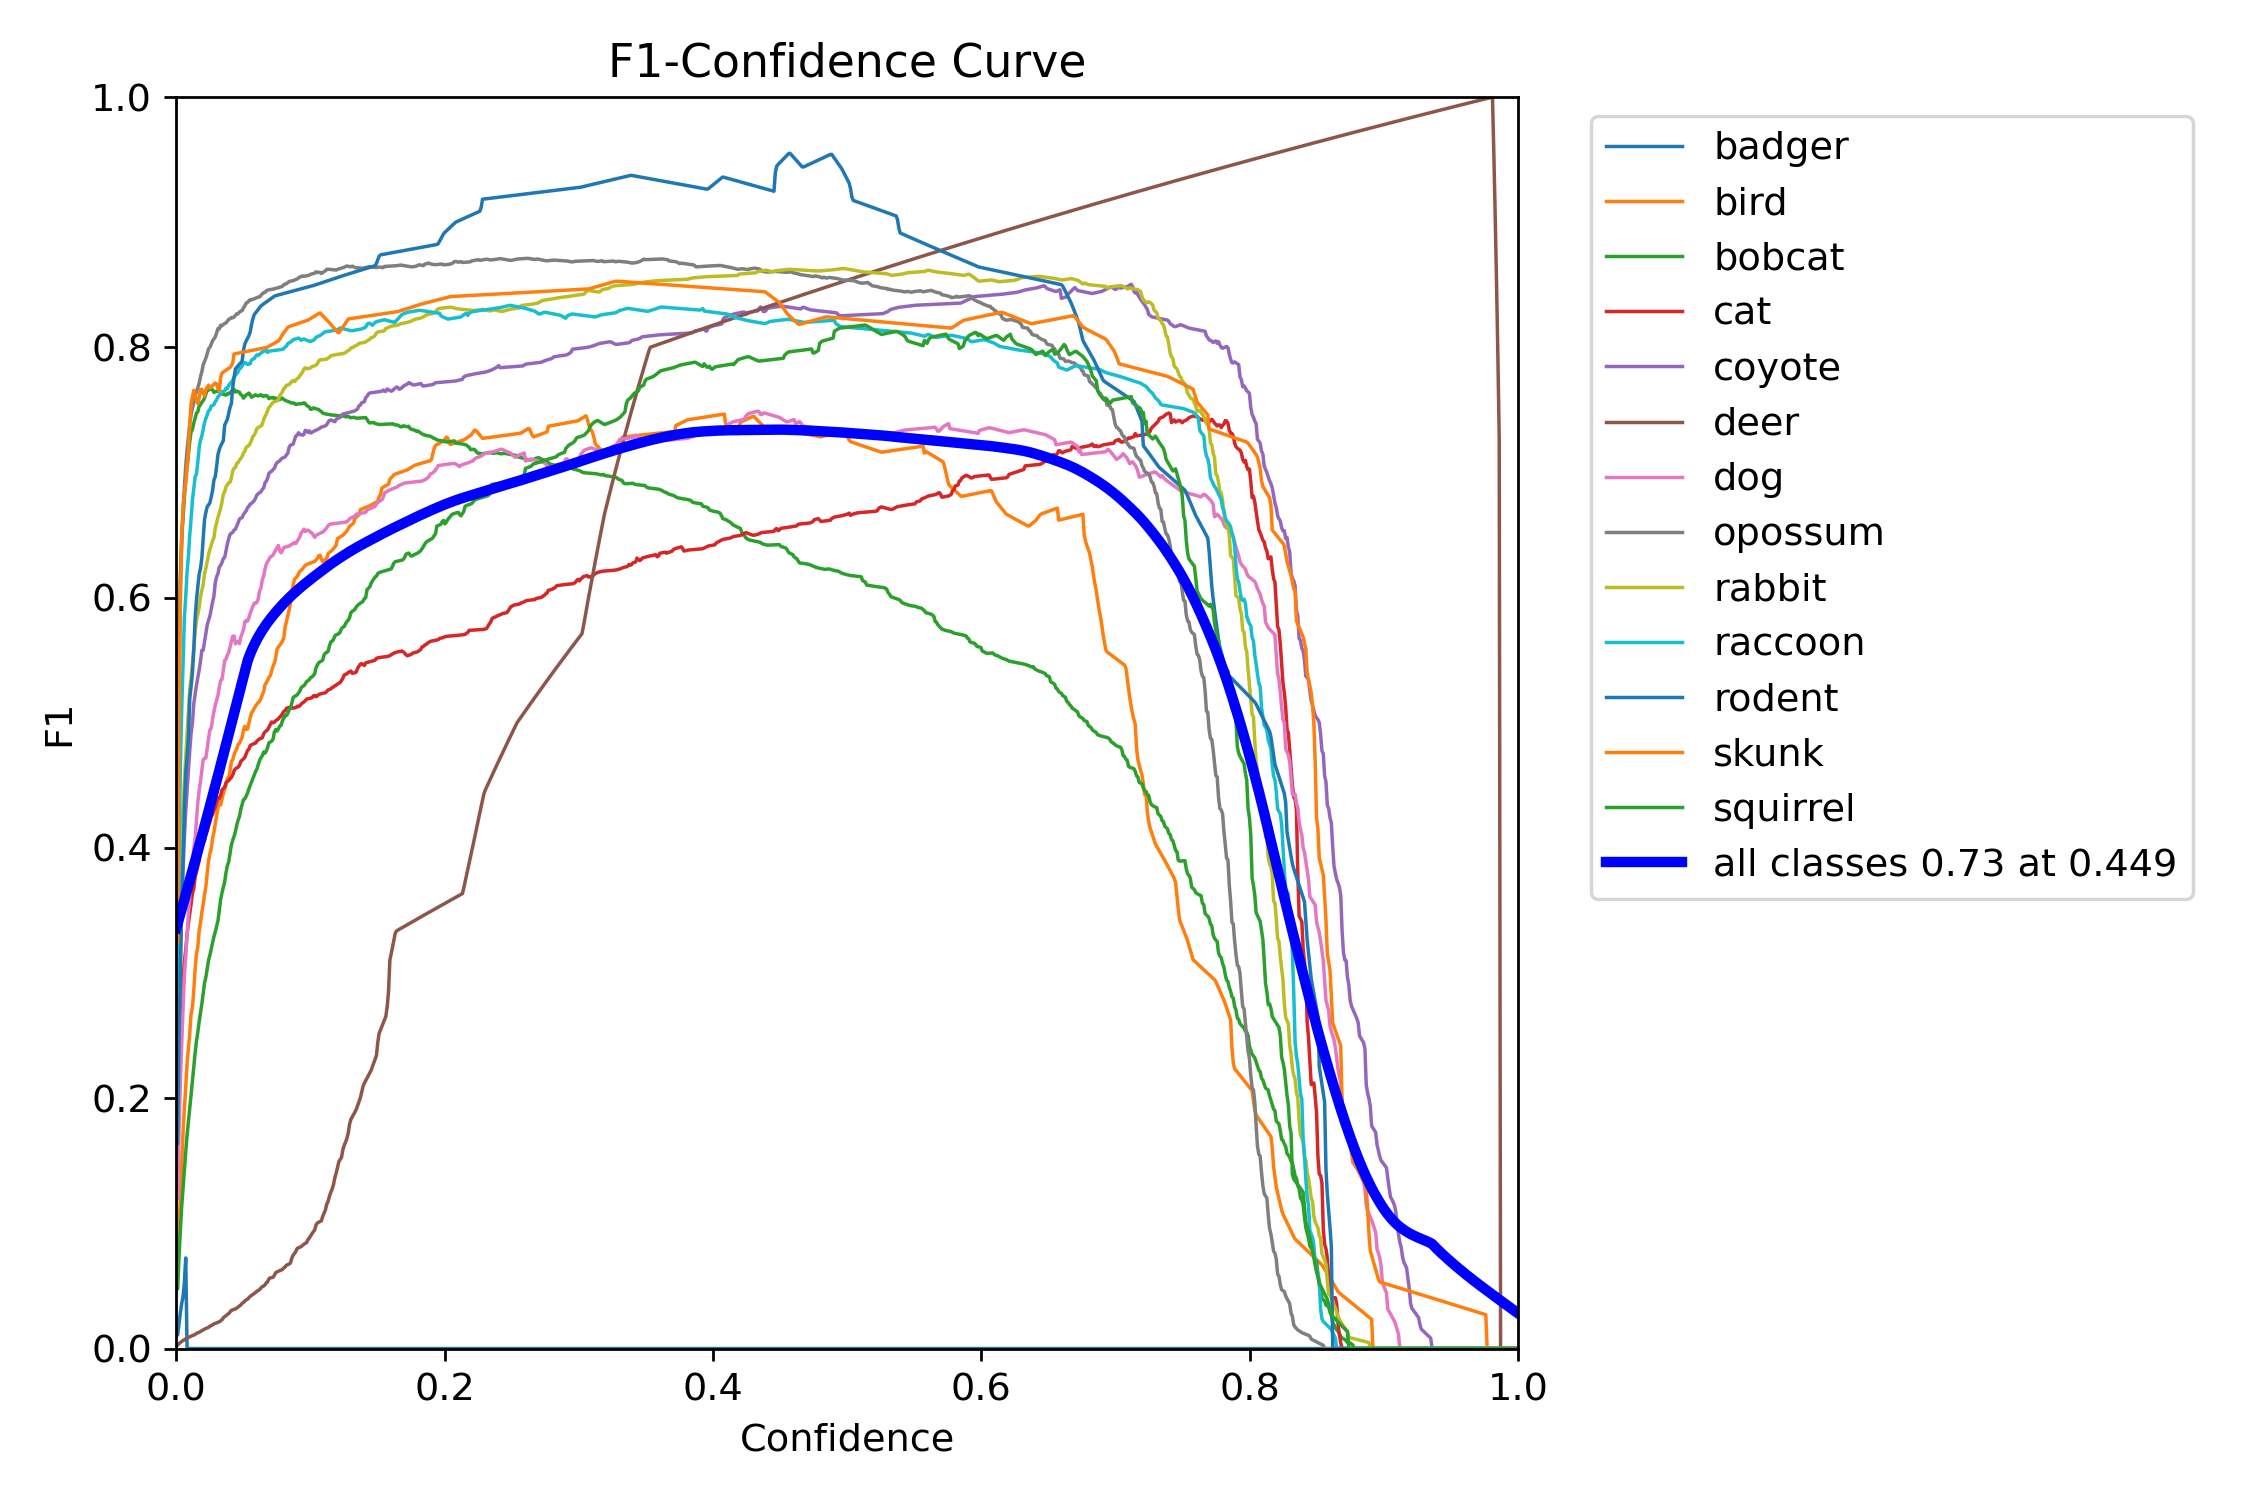
\includegraphics[width=0.75\linewidth]{figuras/f1_validacion.png}
  \caption{Curva F1--confianza de E3 en validación. El máximo promedio
  ($F1=0{,}73$) se alcanza en 0,45 y la curva es plana entre 0,4 y 0,6.}
\end{figure}

\section{Ejemplos de la prueba de borrado}

\begin{figure}[h]
  \centering
  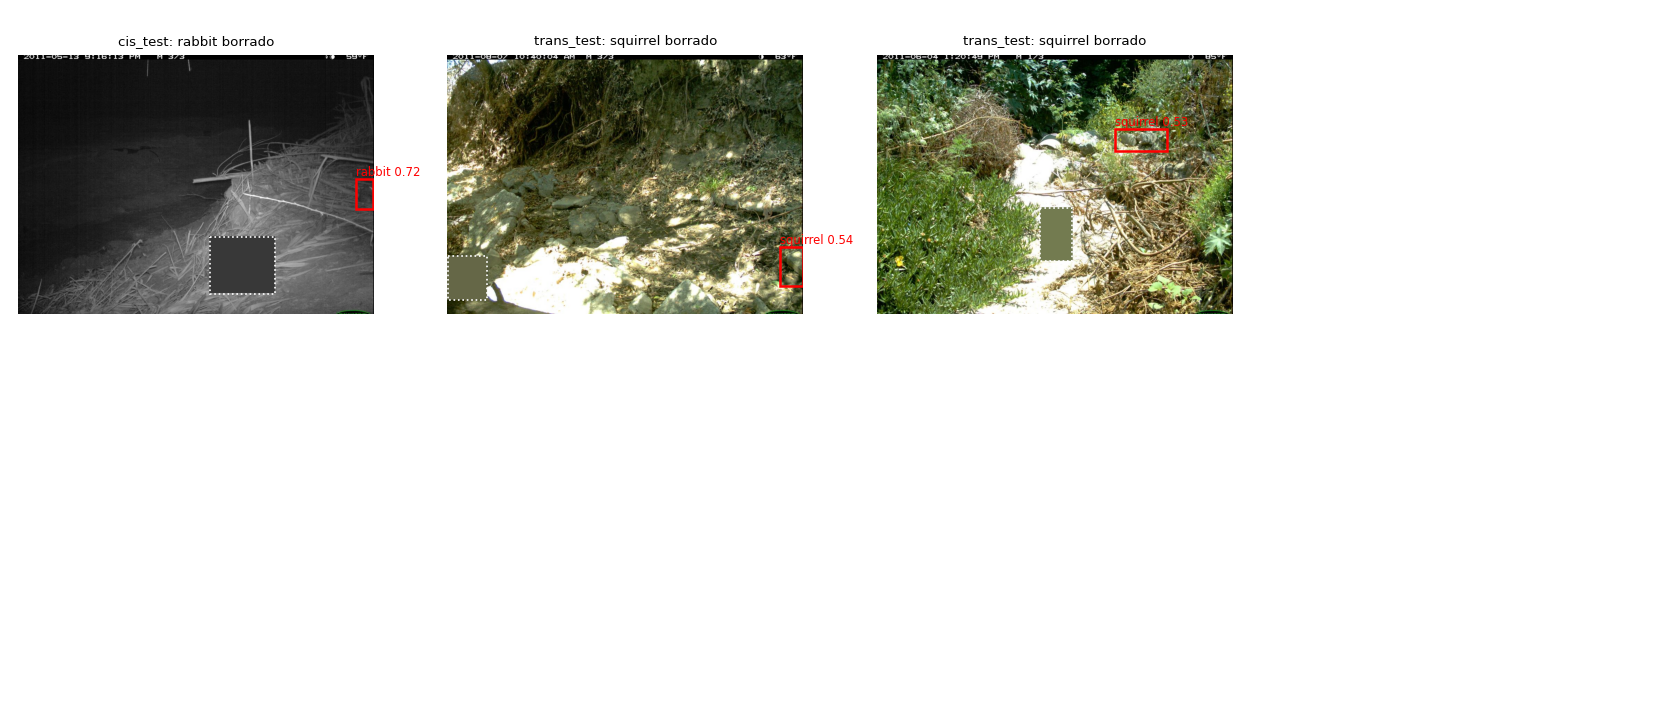
\includegraphics[width=\linewidth]{figuras/borrado_ejemplos.png}
  \caption{Los pocos casos en que, tras borrar al animal (rectángulo punteado),
  el modelo vuelve a predecir la misma especie.}
\end{figure}

\section{Recall por tamaño de caja}

\begin{figure}[h]
  \centering
  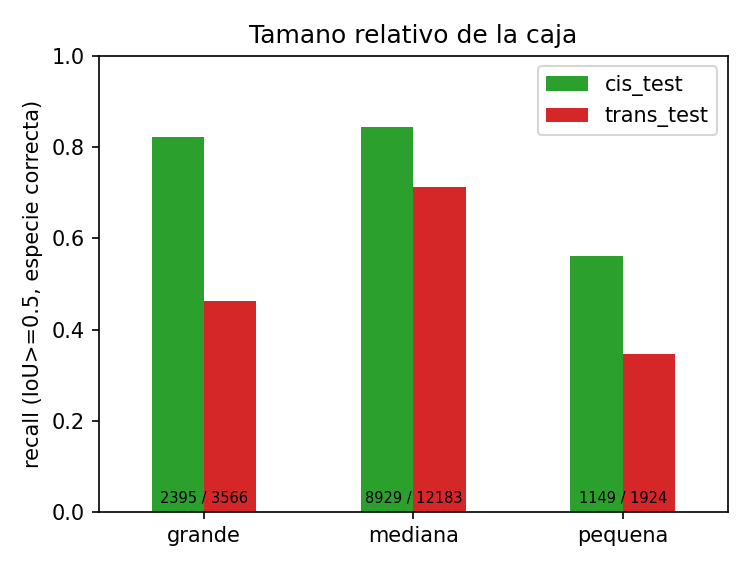
\includegraphics[width=0.8\linewidth]{figuras/recall_tamano.png}
  \caption{Recall (IoU $\geq 0{,}5$, especie correcta) por tamaño de caja en
  \texttt{cis\_test} (verde) y \texttt{trans\_test} (rojo).}
\end{figure}

\end{document}
